\documentclass[11pt, a4paper,oneside,chapterprefix=false]{scrbook}

\usepackage{a4wide}
\usepackage{times}
\usepackage{helvet}   % sets sans serif font

\usepackage{amsmath,amssymb,amsthm}

\usepackage{graphicx}
\usepackage{subfigure}  
\usepackage{fancybox} % for shadowed or double bordered boxes
\usepackage{fancyhdr}
\usepackage{mdframed}
\usepackage{pdflscape}

\DeclareGraphicsExtensions{.pdf, .jpg}

%% macros
 \def\mathbi#1{\textbf{\em #1}}
 
% commands
\newcommand{\Adjoint}{\mbox{\rm Adj}}
\newcommand{\Area}{\mbox{\rm Area}}
\newcommand{\ACos}{{\mbox{\rm Cos}^{-1}}}
\newcommand{\ASin}{{\mbox{\rm Sin}^{-1}}}
\newcommand{\ATan}{{\mbox{\rm atan2}}}
\newcommand{\Code}[1]{{\tt #1}}
\newcommand{\Complex}{\mbox{\bf C}}
\newcommand{\Cross}{{\mbox{\rm Cross}}}
\newcommand{\Mydddot}[1]{\mbox{\shortstack{$.$\hspace*{-1pt}$.$\hspace*{-1pt}$.$\\$#1$}}}
\newcommand{\Degree}{\mbox{\rm degree}}
\newcommand{\Diag}{\mbox{\rm Diag}}
\newcommand{\Dim}{\mbox{\rm dim}}
\newcommand{\Dist}{\mbox{\rm Distance}}
\newcommand{\IntTwo}{\int\!\!\int}
\newcommand{\IntThree}{\int\!\!\int\! \!\int}
\newcommand{\Kernel}{\mbox{\rm kernel}}
\newcommand{\Kross}{\mbox{\rm Kross}}
\newcommand{\Grad}{\nabla}
\newcommand{\Perp}{\mbox{\rm Perp}}
\newcommand{\Point}[1]{{\cal #1}}
\newcommand{\Rank}{\mbox{\rm rank}}
\newcommand{\Range}{\mbox{\rm range}}
\newcommand{\Real}{{\mbox{\rm I}\hspace*{-2pt}\mbox{\rm R}}}
\newcommand{\RealSbt}{{\mbox{\rm\scriptsize I}\hspace*{-2pt}\mbox{\rm\scriptsize R}}}
\newcommand{\Res}{\mbox{\rm resultant}}
\newcommand{\Sbt}[1]{{\mbox{\rm\scriptsize #1}}}
\newcommand{\MySign}{\mbox{\rm Sign}}
\newcommand{\SignSBT}{\mbox{\rm\scriptsize Sign}}
\newcommand{\Skew}{\mbox{\rm Skew}}
\newcommand{\Span}{\mbox{\rm Span}}
\newcommand{\SqrDist}{\mbox{\rm Distance$^2$}}
\newcommand{\Trace}{\mbox{\rm Trace}}
\newcommand{\TRN}{{\mbox{\rm\scriptsize T}}}
\newcommand{\Vector}[1]{\mbox{\bf #1}}
\newcommand{\VectorM}[1]{\mbox{\boldmath $#1$}}
\newcommand{\Volume}{\mbox{\rm Volume}}

\newcommand{\IVec}{\mbox{\boldmath $\imath$}}
\newcommand{\JVec}{\mbox{\boldmath $\jmath$}}
\newcommand{\KVec}{\mbox{\boldmath $k$}}
\newcommand{\LVec}{\mbox{\boldmath $\ell$}}
\newcommand{\RMat}{{\cal R}}
\newcommand{\QMat}{{\cal Q}}
\newcommand{\QCMat}{\overline{\cal Q}}

\newcommand{\Lerp}{\mbox{\rm lerp}}
\newcommand{\Slerp}{\mbox{\rm slerp}}
\newcommand{\Quad}{\mbox{\rm quad}}
\newcommand{\Squad}{\mbox{\rm squad}}

\newcommand{\ODer}[2]{\frac{d #1}{d #2}}
\newcommand{\ODerT}[2]{\frac{d^2 #1}{d {#2}^2}}
\newcommand{\ODerM}[3]{\frac{d #1}{d #2 \, d #3}}
\newcommand{\PDer}[2]{\frac{\partial #1}{\partial #2}}
\newcommand{\PDerT}[2]{\frac{\partial^2 #1}{\partial {#2}^2}}
\newcommand{\PDerM}[3]{\frac{\partial^2 #1}{\partial #2 \, \partial #3}}

% mass density symbol
\newcommand{\Den}{\delta}

% environments
\newenvironment{BArray}[1]{\left\{ \begin{array}{#1}}{\end{array} \right\}}
\newenvironment{Combin}{\left( \begin{array}{c}}{\end{array} \right)}
\newenvironment{Matrix}[1]{\left[ \begin{array}{#1}}{\end{array} \right]}


\let\mbf=\mathbf
\let\mvec=\mathbf
\let\mcal=\mathcal
\let\mfunc=\mathrm

%\def\R{\mbox{\ensuremath{\mathrm{I\!R}}}}
\newcommand{\R}{\ensuremath{\mathbb{R}}}
\newcommand{\N}{\ensuremath{\mathbb{N}}}
\newcommand{\Z}{\ensuremath{\mathbb{Z}}}
\newcommand{\C}{\ensuremath{\mathbb{C}}}

\newcommand{\of}[1]{\left( #1 \right)}
\newcommand{\abs}[1]{\left| #1 \right|}
\newcommand{\norm}[1]{\left\Vert {#1} \right\Vert}
\newcommand{\gradient}[1]{\nabla{\!}_{#1}{\,}}
\newcommand{\twovec}[2]{\left( #1 \atop #2 \right)}
\newcommand{\threevec}[3]{\left(\begin{array}{c}#1\\#2\\#3\end{array}\right)}
\newcommand{\fourvec}[4]{\left(\begin{array}{c}#1\\#2\\#3\\#4\end{array}\right)}

\newcommand{\refsec}[1]{Section~\ref{sec:#1}}
\newcommand{\reffig}[1]{Fig.~\ref{fig:#1}}
\newcommand{\reftab}[1]{Tab.~\ref{tab:#1}}
\newcommand{\refeq}[1]{Eq.~(\ref{eq:#1})}

%\newcommand{\R}{\hspace*{0.1ex}{\sf I} \hspace{-0.3ex}{\sf R}}

%6.5
\newcommand{\eps}{\mbox{$\epsilon$}}
\newcommand{\dmin}{\mbox{$d_{\min}$}}
\newcommand{\dmax}{\mbox{$d_{\max}$}}
\newcommand{\dminmax}{\mbox{$[\dmin,\dmax]$}}

%4.2:
\def\M{\mathcal{M}}
\def\n{\mathbi{n}}
\def\p{\mathbi{p}}
\def\q{\mathbi{q}}
\def\x{\mathbi{x}}
\def\tp{^{\mathsf{T}}}

\let\vec=\mathbi%
\let\mat=\mathbf%
\let\set= \mathcal%

% Taken from (and slightly modified): http://stackoverflow.com/questions/741985/latex-source-code-listing-like-in-professional-books

\usepackage{listings}
\usepackage{courier}
\usepackage{color}
\definecolor{lightgray}{gray}{0.9}
\definecolor{commentgreen}{rgb}{0.2,0.56,0.2}
 \lstset{
         basicstyle=\footnotesize\ttfamily, % Standardschrift
         numbers=left,               % Ort der Zeilennummern
         numberstyle=\tiny,          % Stil der Zeilennummern
         %stepnumber=2,               % Abstand zwischen den Zeilennummern
         numbersep=5pt,              % Abstand der Nummern zum Text
         tabsize=2,                  % Groesse von Tabs
         extendedchars=true,         %
         breaklines=true,            % Zeilen werden Umgebrochen
         keywordstyle=\color{red},
                frame=b,         
          keywordstyle=[1]\textbf,    % Stil der Keywords
         keywordstyle=[2]\textbf,    %
         keywordstyle=[3]\textbf,    %
         keywordstyle=[4]\textbf,   %\sqrt{\sqrt{}} %
         stringstyle=\color{blue}\ttfamily, % Farbe der String
         showspaces=false,           % Leerzeichen anzeigen ?
         showtabs=false,             % Tabs anzeigen ?
         xleftmargin=17pt,
         framexleftmargin=17pt,
         framexrightmargin=5pt,
         framexbottommargin=4pt,
         backgroundcolor=\color{lightgray},
         showstringspaces=false,      % Leerzeichen in Strings anzeigen ?
         commentstyle=\color{commentgreen}
 }
 \lstloadlanguages{% Check Dokumentation for further languages ...
         %[Visual]Basic
         %Pascal
         %C
		PHP, 
         C++
         %XML
         %HTML
         %Java
 }
    %\DeclareCaptionFont{blue}{\color{blue}} 

  %\captionsetup[lstlisting]{singlelinecheck=false, labelfont={blue}, textfont={blue}}
  \usepackage{caption}
\DeclareCaptionFont{white}{\color{white}}
\DeclareCaptionFormat{listing}{\colorbox[cmyk]{0.43, 0.35, 0.35,0.01}{\parbox{\textwidth}{\hspace{15pt}#1#2#3}}}
\captionsetup[lstlisting]{format=listing,labelfont=white,textfont=white, singlelinecheck=false, margin=0pt, font={bf,footnotesize}}

\usepackage{color}
\usepackage{hyperref}
\definecolor{RED}{rgb}{1,0,0}
\definecolor{GREEN}{rgb}{0,0.7,0}
\definecolor{BLUE}{rgb}{0,0,1}
\definecolor{Orange}{rgb}{0.7,0.7,0.7}
\newcommand{\FIXME}[1]{{\color{RED}{\textbf{FIX}: #1}}}

\addtolength{\textheight}{2.0cm}
\addtolength{\voffset}{-1cm}
\addtolength{\textwidth}{1.8cm}
\addtolength{\hoffset}{-.9cm}

\widowpenalty=10000
\clubpenalty=10000

%\author{Hans Muster}
%\title{Blockwise Hierarchical Data Decompositions}
%\date{Fall Semester 2011}

\begin{document}

\frontmatter
%\maketitle %automatic version
% --- selfmade version ----
\begin{titlepage}
	\setlength{\parindent}{0cm}
	\addtolength{\textheight}{1.0cm}

	\vspace{0.5cm}
	\Huge
	{\textbf \textsf{VIAN\\ \huge Datamodel and XML Export Format}}

	\vfill\vfill\vfill
	\vfill
	\includegraphics*[width=1.0\textwidth]{figures/vian_02.png}
	\vfill \vfill \vfill
	\large
	Author:\\
	Gaudenz Halter, 27.06.2018\\
	
	
	
	


	\begin{minipage}[b]{0.5\textwidth}
	ERC Advanced Grant FilmColors\\
	Department of Film Studies \\
	University of Z{\"u}rich
	\end{minipage}
	%
	\begin{minipage}[b]{0.5\textwidth} \raggedleft
	Visualization and MultiMedia Lab \\
	Department of Informatics \\
	University of Z{\"u}rich
	\end{minipage}

	\vfill
	\hrule
	\vspace{0.5cm}
	\includegraphics*[width=0.3\textwidth]{figures/uzh_logo} \hfill
	\includegraphics*[width=0.3\textwidth]{figures/vmml_logo}

\end{titlepage}
%%


\begin{landscape}
	\begin{figure}[htp]
		\centering
		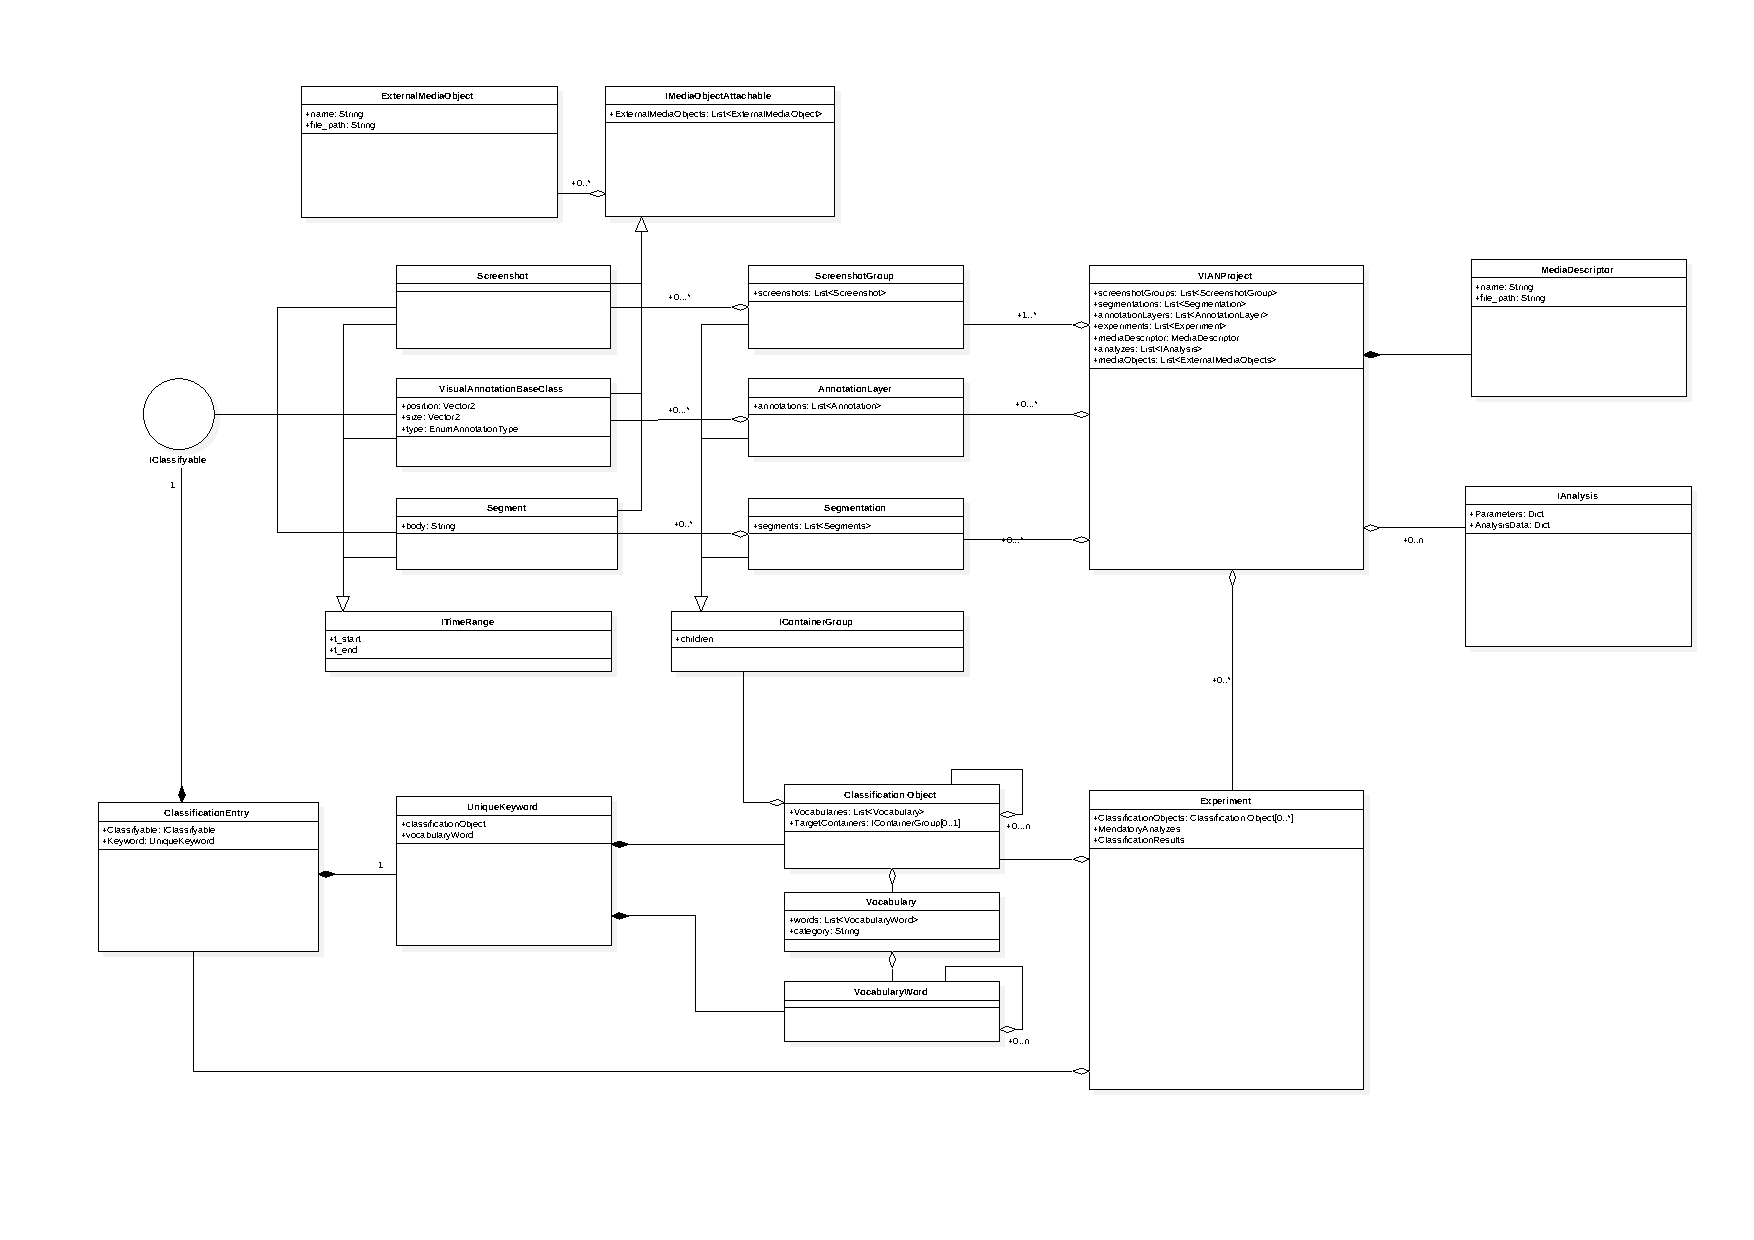
\includegraphics[width = 1.5\textwidth]{figures/VIAN_DataModel_simplified.pdf}
		\label{fig:vian_classobj}
	\end{figure}
\end{landscape}

\section{Introduction}
VIAN projects are serialized into a json file and a list of binary objects, holding large numeric data generated during analysis. (i.e. Color Palettes, Histograms, etc.)\\

Since a lot of the data stored is application and python specific, VIAN supports an XML export of annotations and analysis, its elements are described in this document. Links between different entities are serialized using the ID attribute. IDs are guaranteed to be unique and declared before referenced in the document.

Additionally the VIAN project json file is described at the end of this document by an example.

\section{XML Schema}
\subsection{Element: ANNOTATION\_DOCUMENT}
\lstinputlisting[language=xml,label=example]{code/edocument.txt}
\subsection{Element: HEADER}
\lstinputlisting[language=xml,label=example]{code/eheader.txt}
\subsection{Element: MEDIA\_DESCRIPTOR}
\lstinputlisting[language=xml,label=example]{code/edescriptor.txt}

\newpage
\subsection{Element: TIME\_ORDER and TIME\_SLOT}
\lstinputlisting[language=xml,label=example]{code/etimeorder.txt}
VIAN uses an implicit timeline, that is, each Segment, Visual Annotation or Screenshot object stores it's media time directly. In the XML export format, a list of TIME\_SLOTS is created, and each serialization of an object media-time information references one or two TIME\_SLOTS. \\
\\
Note: Currently TIME\_SLOTS are unique, thus for each time there can not be more than one TIME\_SLOT.\\
\subsection{Element: SEGMENTATION and SEGMENT}
\lstinputlisting[language=xml,label=example]{code/esegmentation.txt}
The first kind of annotation supported by VIAN are called "Segment" and are aggregated in a Tier called "Segmentation". A segment has a start and end-point and may have a text body. \\

\subsection{Element: SCREENSHOTS and SCREENSHOT}
\lstinputlisting[language=xml,label=example]{code/escreenshots.txt}
The second type of annotations are "Screenshots", which are aggregated in "ScreenshotGroups". 
A screenshot only has a start-time in the XML export. 

\newpage
\subsection{Element: ANNOTATION\_LAYER and VISUAL\_ANNOTATION}
Finally there are "Visual Annotations", aggregated in "Annotation Layers", which represent vector graphics, that are placed on the screen. \\
\lstinputlisting[language=xml,label=example]{code/evisannotation.txt}
Note that the export of visual annotations does currently not support: 
\begin{itemize}
	\item Export of keys on annotations
	\item Export of FreeHand annotations. 
\end{itemize}


\newpage
\subsection{Element: EXPERIMENT}
The process of data acquisition (i.e. creating segments, annotations and screenshots) and classification of these entities using vocabularies is splitted, such that different classifications can be performed on the same segments and annotations. \\ 
Essentially a subject of interest (Classification Object), can be present in several tiers (the targets), and can be classified by multiple vocabularies. For each classification object a list of unique keywords is generated which can then be attached to the classification targets as tags. All this information is contained in an experiment.\\

\centering
\begin{minipage}{0.8\textwidth}
\textbf{Example:}
	The classification object "Background" can be present in the scene segmentation as well as the screenshots, 
	and would probably be classified with the vocabularies "Color", "Shadows". 
\end{minipage}
\lstinputlisting[language=xml,label=example]{code/eexperiment.txt}

\subsection{Element: CLASSIFICATION\_OBJECT}
\lstinputlisting[language=xml,label=example]{code/eclassificationobj.txt}

\subsection{Element:VOCABULARY and VOCABULARY\_WORD}
\lstinputlisting[language=xml,label=example]{code/evocabulary.txt}

\subsection{Element: KEYWORDS}
\lstinputlisting[language=xml,label=example]{code/ekeywords.txt}

\subsection{Element: CLASSIFICATION}
The classification represents the mapping of tags their targets. (screenshots, segments, visual annotations) 
\lstinputlisting[language=xml,label=example]{code/eclassification.txt}
\newpage

\subsection{Element: EXTERNAL\_MEDIA\_OBJECT}
\lstinputlisting[language=xml,label=example]{code/eexternalmedia.txt}

\subsection{Element: ANALYSES}
\lstinputlisting[language=xml,label=example]{code/eanalyses.txt}


\newpage
\section{Json Schema}
VIAN serializes its projects into a folder hierarchy and a Json file. Since this contains a lot of application specific information and has never been intended to be read by other applications, the XML Export may be the better way enforce interoperability with other applications. But for the sake of completeness, a documented Json is shown in the rest of this document. 
\lstinputlisting[language=c++,label=example]{code/bladerunner.eext}

\end{document}
